\section{Anhang}
\subsection{Diagramme und Grafiken}
\subsubsection{Vergleich: DLD Aufwand vs QGram Aufwand mit Fuzzy Join}
\subsubsection{Vergleich: Theoretischer DLD vs QGram Zeitvergleich }
\subsubsection{Use-Case QGJoin}
\begin{figure}
	\caption{Use-Case Diagramm des QGJoin Programms}
	\label{fig:qgjoinUseCase}
	\includegraphics[width=\textwidth]{qgjoin_usecase}
\end{figure}

\subsubsection{Geschäftslogik Alt}
\begin{figure}
	\caption{UML Diagramm der bisherigen Geschäftslogik}
	\label{fig:geschäftslogikAlt}
\end{figure}



\subsubsection{Aktivitätsdiagramm: Programmlogik}
\begin{figure}[!htp]
	\caption{Programmlogik als UML Aktivitätsdiagramm}
	\label{fig:programmlogik}
	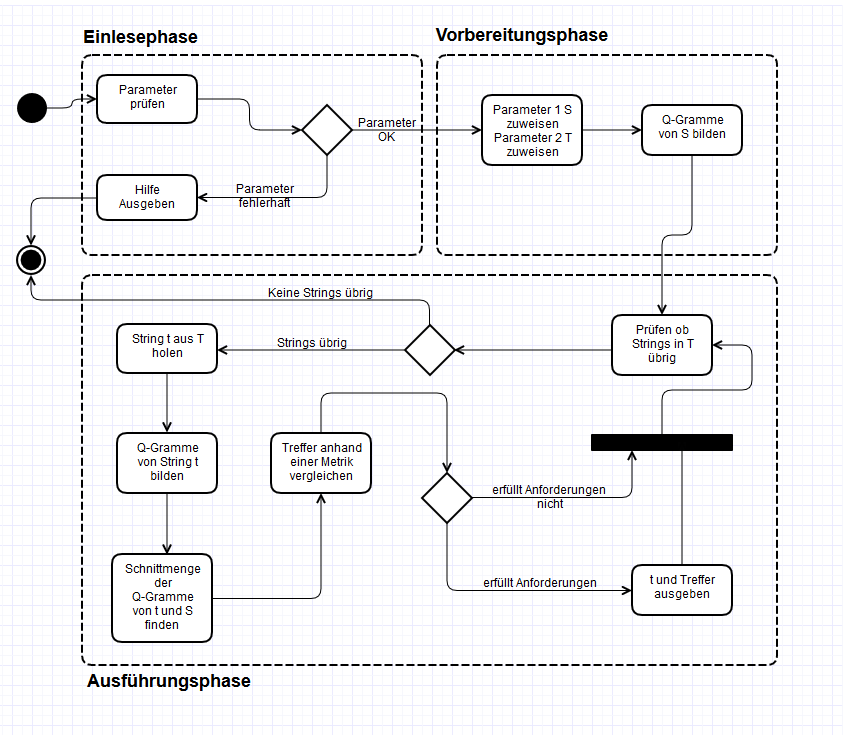
\includegraphics[width=\textwidth]{algo}
	\centering
\end{figure}

\subsubsection{Projektstruktur}
\begin{figure}[!htp]
	\caption{Übersicht der Projektstruktur}
	\label{fig:folderstruct}
	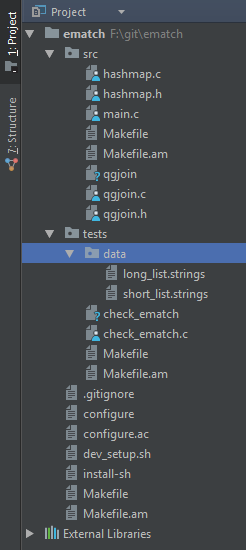
\includegraphics[width=\textwidth]{folder_struct}
\end{figure}

\subsubsection{Analyse: Verteilung der Qgramme}
\begin{figure}[!htp]
    \caption{Verteilung der QGramme im zu bearbeitenden Datensatz}
    \label{fig:qgram_verteilung}
    \includegraphics[width=\textwidth]{multiplicity_of_qgrams.eps}
    \centering
\end{figure}

\subsubsection{Datenmodell}
\begin{figure}[!htp]
    \caption{UML Darstellung des Datenmodells}
    \label{fig:datenmodell}
    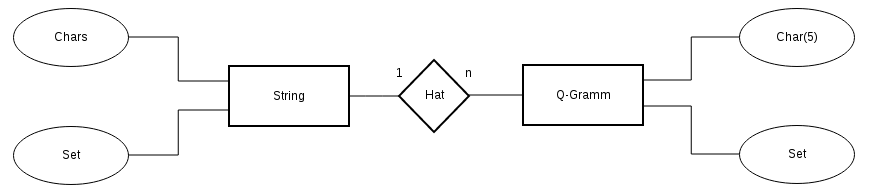
\includegraphics[width=\textwidth]{datenmodell}
    \centering
\end{figure}



\subsection{Tabellen}
\subsubsection{Projektkosten}
\begin{sidewaystable}
	\centering
	\caption{Projektkosten}
	\label{tabelle:projektkosten}
	\begin{tabular}{llllll}
		\rowcolor[HTML]{9698ED}
		{\color[HTML]{FFFFFF} \textbf{Vorgang}} & {\color[HTML]{FFFFFF} \textbf{Mitarbeiter}} & {\color[HTML]{FFFFFF} \textbf{Stunden}} & {\color[HTML]{FFFFFF} \textbf{Personal}} & {\color[HTML]{FFFFFF} \textbf{Ressources}} & {\color[HTML]{FFFFFF} \textbf{Gesamt}} \\
		Entwicklungskosten                      & 1                                           & 70                                      & 385.00 €                                 & 1,295.00 €                                 & 1,680.00 €                             \\
		\rowcolor[HTML]{BBDAFF}
		Fachgespräch                            & 2                                           & 5                                       & 350.00 €                                 & 92.50 €                                    & 1,842.50 €                             \\
		Code Review                             & 2                                           & 2                                       & 140.00 €                                 & 37.00 €                                    & 317.00 €                               \\
		\rowcolor[HTML]{BBDAFF}
		Abnahme                                 & 2                                           & 0.5                                     & 35.00 €                                  & 9.25 €                                     & 44.25 €                                \\
		&                                             &                                         & \multicolumn{2}{l}{\textbf{Projektkosten Gesamt:}}                                    & \textbf{3,883.75 €}
	\end{tabular}
\end{sidewaystable}

\subsubsection{Nutzwertanalyse: Projektentwicklung}
\begin{sidewaystable}
	\centering
	\caption{Nutzwertanalyse Projektentwicklung}
	\label{nwa:projektentwicklung}
	\begin{tabular}{llllllllll}
		\rowcolor[HTML]{9698ED}
		{\color[HTML]{FFFFFF} \textbf{Kriterien}} & {\color[HTML]{FFFFFF} \textbf{Gewicht}} & {\color[HTML]{FFFFFF} \textbf{Externe Entwicklung}} & {\color[HTML]{FFFFFF} \textbf{}}       & {\color[HTML]{FFFFFF} \textbf{Interne Entwicklung}} & {\color[HTML]{FFFFFF} \textbf{}}       & {\color[HTML]{FFFFFF} \textbf{Dedizierter 12-Kerner}} & {\color[HTML]{FFFFFF} \textbf{}}       & {\color[HTML]{FFFFFF} \textbf{Cluster}}   & {\color[HTML]{FFFFFF} \textbf{}}       \\
		\rowcolor[HTML]{9698ED}
		{\color[HTML]{FFFFFF} \textbf{}}          & {\color[HTML]{FFFFFF} \textbf{}}        & {\color[HTML]{FFFFFF} \textbf{Bewertung}}           & {\color[HTML]{FFFFFF} \textbf{Gesamt}} & {\color[HTML]{FFFFFF} \textbf{Bewertung}}           & {\color[HTML]{FFFFFF} \textbf{Gesamt}} & {\color[HTML]{FFFFFF} \textbf{Bewertung}}             & {\color[HTML]{FFFFFF} \textbf{Gesamt}} & {\color[HTML]{FFFFFF} \textbf{Bewertung}} & {\color[HTML]{FFFFFF} \textbf{Gesamt}} \\
		Projektkosten                             & 45.00\%                                 & 4                                                   & 1.8                                    & 5                                                   & 2.25                                   & 4                                                     & 1.8                                    & 3                                         & 1.35                                   \\
		\rowcolor[HTML]{BBDAFF}
		Nachhaltigkeit                            & 15.00\%                                 & 4                                                   & 0.6                                    & 4                                                   & 0.6                                    & 1                                                     & 0.15                                   & 1                                         & 0.15                                   \\
		Flexibilität                              & 5.00\%                                  & 3                                                   & 0.15                                   & 5                                                   & 0.25                                   & 4                                                     & 0.2                                    & 4                                         & 0.2                                    \\
		\rowcolor[HTML]{BBDAFF}
		Unterhaltskosten                          & 35.00\%                                 & 4                                                   & 1.4                                    & 4                                                   & 1.4                                    & 2                                                     & 0.7                                    & 1                                         & 0.35                                   \\
		\textbf{Gesamt}                           & \textbf{100.00\%}                       & \textbf{}                                           & \textbf{3.95}                          & \textbf{}                                           & \textbf{4.5}                           & \textbf{}                                             & \textbf{2.85}                          & \textbf{}                                 & \textbf{2.05}
	\end{tabular}
\end{sidewaystable}

\subsubsection{Nutzwertanalyse: Programmiersprachen}

\begin{sidewaystable}
	\centering
	\caption{Nutzwertanalyse der Programmiersprachen}
	\label{nwa:sprachen}
	\begin{tabular}{llllllllll}
		\rowcolor[HTML]{9698ED}
		{\color[HTML]{FFFFFF} \textbf{Kriterien}} & \multicolumn{1}{c}{\cellcolor[HTML]{9698ED}{\color[HTML]{FFFFFF} \textbf{Gewicht}}} & \multicolumn{2}{c}{\cellcolor[HTML]{9698ED}{\color[HTML]{FFFFFF} \textbf{C}}}                                                                                              & \multicolumn{2}{c}{\cellcolor[HTML]{9698ED}{\color[HTML]{FFFFFF} \textbf{C++}}}                                                                                            & \multicolumn{2}{c}{\cellcolor[HTML]{9698ED}{\color[HTML]{FFFFFF} \textbf{Java}}}                                                                                           & \multicolumn{2}{c}{\cellcolor[HTML]{9698ED}{\color[HTML]{FFFFFF} \textbf{Haskell}}}                                                                                        \\
		\rowcolor[HTML]{9698ED}
		{\color[HTML]{FFFFFF} \textbf{}}          & \multicolumn{1}{c}{\cellcolor[HTML]{9698ED}{\color[HTML]{FFFFFF} \textbf{}}}        & \multicolumn{1}{c}{\cellcolor[HTML]{9698ED}{\color[HTML]{FFFFFF} \textbf{Bewertung}}} & \multicolumn{1}{c}{\cellcolor[HTML]{9698ED}{\color[HTML]{FFFFFF} \textbf{Gesamt}}} & \multicolumn{1}{c}{\cellcolor[HTML]{9698ED}{\color[HTML]{FFFFFF} \textbf{Bewertung}}} & \multicolumn{1}{c}{\cellcolor[HTML]{9698ED}{\color[HTML]{FFFFFF} \textbf{Gesamt}}} & \multicolumn{1}{c}{\cellcolor[HTML]{9698ED}{\color[HTML]{FFFFFF} \textbf{Bewertung}}} & \multicolumn{1}{c}{\cellcolor[HTML]{9698ED}{\color[HTML]{FFFFFF} \textbf{Gesamt}}} & \multicolumn{1}{c}{\cellcolor[HTML]{9698ED}{\color[HTML]{FFFFFF} \textbf{Bewertung}}} & \multicolumn{1}{c}{\cellcolor[HTML]{9698ED}{\color[HTML]{FFFFFF} \textbf{Gesamt}}} \\
		Performanz                                & 30.00\%                                                                             & 5                                                                                     & 1.5                                                                                & 5                                                                                     & 1.5                                                                                & 4                                                                                     & 1.2                                                                                & 5                                                                                     & 1.5                                                                                \\
		\rowcolor[HTML]{BBDAFF}
		Speichereffizienz                         & 30.00\%                                                                             & 5                                                                                     & 1.5                                                                                & 5                                                                                     & 1.5                                                                                & 3                                                                                     & 0.9                                                                                & 4                                                                                     & 1.2                                                                                \\
		Dokumentation                             & 20.00\%                                                                             & 5                                                                                     & 1                                                                                  & 4                                                                                     & 0.8                                                                                & 4                                                                                     & 0.8                                                                                & 2                                                                                     & 0.4                                                                                \\
		\rowcolor[HTML]{BBDAFF}
		Systemische Vorraussetzungen              & 10.00\%                                                                             & 5                                                                                     & 0.5                                                                                & 5                                                                                     & 0.5                                                                                & 3                                                                                     & 0.3                                                                                & 3                                                                                     & 0.3                                                                                \\
		Datenstrukturen                           & 10.00\%                                                                             & 3                                                                                     & 0.3                                                                                & 4                                                                                     & 0.4                                                                                & 5                                                                                     & 0.5                                                                                & 5                                                                                     & 0.5                                                                                \\
		\rowcolor[HTML]{BBDAFF}
		\textbf{Gesamt}                           & \textbf{100.00\%}                                                                   & \textbf{}                                                                             & \textbf{4.8}                                                                       & \textbf{}                                                                             & \textbf{4.7}                                                                       & \textbf{}                                                                             & \textbf{3.7}                                                                       & \textbf{}                                                                             & \textbf{3.9}
	\end{tabular}
\end{sidewaystable}

\subsubsection{Nutzwertanalyse: Datentyp der Menge Q}
\begin{sidewaystable}
	\centering
	\caption{Nutzwertanalyse der Datentypen für Q}
	\label{nwa:datentyp}
	\begin{tabular}{llllll}
		\rowcolor[HTML]{9698ED}
		\cellcolor[HTML]{9698ED}{\color[HTML]{FFFFFF} }                                     & \cellcolor[HTML]{9698ED}{\color[HTML]{FFFFFF} }                                   & \multicolumn{2}{l}{\cellcolor[HTML]{9698ED}{\color[HTML]{FFFFFF} \textbf{Hashmap}}} & \multicolumn{2}{l}{\cellcolor[HTML]{9698ED}{\color[HTML]{FFFFFF} \textbf{Binärbaum}}} \\
		\rowcolor[HTML]{9698ED}
		\multirow{-2}{*}{\cellcolor[HTML]{9698ED}{\color[HTML]{FFFFFF} \textbf{Kriterien}}} & \multirow{-2}{*}{\cellcolor[HTML]{9698ED}{\color[HTML]{FFFFFF} \textbf{Gewicht}}} & {\color[HTML]{FFFFFF} \textbf{Bewertung}}  & {\color[HTML]{FFFFFF} \textbf{Gesamt}} & {\color[HTML]{FFFFFF} \textbf{Bewertung}}   & {\color[HTML]{FFFFFF} \textbf{Gesamt}}  \\
		Speicheraufwand                                                                     & 25.00\%                                                                           & 2                                          & 0.5                                    & 2                                           & 0.5                                     \\
		\rowcolor[HTML]{BBDAFF}
		Schnelligkeit Daten Einfügen (Insert                                                & 20.00\%                                                                           & 5                                          & 1                                      & 4                                           & 0.8                                     \\
		Schnelligkeit Auslesen (Look-up)                                                    & 55.00\%                                                                           & 5                                          & 2.75                                   & 4                                           & 2.2                                     \\
		\rowcolor[HTML]{BBDAFF}
		\textbf{Gesamt}                                                                     & \textbf{100.00\%}                                                                 & \textbf{}                                  & \textbf{4.25}                          & \textbf{}                                   & \textbf{3.5}
	\end{tabular}
\end{sidewaystable}

\subsection{Auszüge}
\subsection{Ressourcen}
\textbf{Hardware}
\begin{itemize}
    \item Büroarbeitsplatz mit vernetztem Rechner
    \item Laptop
\end{itemize}

\textbf{Software}
\begin{itemize}
    \item openSuSE 13.1 - Linux Distribution
    \item Atom IDE - Modulare, Open-Source Entwicklungsumgebung für eine Vielfalt an Sprachen
    \item PyCharm Community Edition - Python Entwicklungsumgebung
    \item LaTeX - Textsatzsystem zur Erstellung von Dokumenten
    \item Python 3.5 - Interpretierte Programmiersprache
    \item Cython - Superset der Python Sprache zur Einbindung von C Code.
    \item GNU Compiler Collection (GCC) - Compilersammlung des GNU Projekts
    \item Git - Dezentralisierte Versionsverwaltung
\end{itemize}

\textbf{Personal}
\begin{itemize}
    \item Mitarbeiter der Abteilung Datenverarbeitung - Festlegung der Anforderungen sowie Abnahme des Projektes
    \item Entwickler - Umsetzung des Projekts
    \item Anwendungsentwickler - Code Review
\end{itemize}


\subsubsection{Lastenheft}
\renewcommand{\labelenumii}{\theenumii}
\renewcommand{\theenumii}{\theenumi.\arabic{enumii}.}
\label{auszug:lastenheft}
\begin{enumerate}
	\item Spezifikationen des Algorithmus
	\begin{enumerate}
		\item Der Algorithmus muss 2 Listen von Strings verarbeiten können,
		wobei eine dieser Listen garantiert in den Speicher passt und die zweite
		eine beliebige Größe haben kann.
		\item Der Algorithmus muss aus der ersten Liste sämtliche Strings finden,
		welche den Strings aus der zweiten Liste ähneln. Die gefundenen Strings
		sollen ausgegeben werden.
		\item Der Algorithmus ist in C zu programmieren.
		\item der Algorithmus verarbeitet 7-Bit ASCII Strings schreibungsunabhängig. Zeichensetzung
		ist beim Vergleich generell zu ignorieren; Ausnahmen bilden die
		Charaktere Bindestrich, Unterstrich und Leerzeichen.
	\end{enumerate}
	\item Spezifikationen des Kommandozeilenprogramms
	\begin{enumerate}
		\item Der Algorithmus muss über die Kommmandozeile ausführbar sein.
		\item Die Erste Liste wird immer als Dateiname übergeben.
		\item Die zweite Liste kann entweder als Dateiname oder über STDIN übergeben werden.
		\item die GNU Standards für Kommandozeilenprogramme müssen eingehalten werden.
		\item Die POSIX Utility Guidelines müssen eingehalten werden.
		\item Das Programm muss unter openSuSE 13.1 laufen.
		\item Alle für das Programm erforderliche Abhängigkeiten
		(z.B. Pakete, Bibliotheken) müssen für openSuSE 13.1 verfügbar sein.
		\item Das Programm muss auf einem einzigen Kern lauffähig sein, und
		darf das laufen auf mehreren Kernen in einem Shared-Memory-Environment
		unterstützen.
		\item Die Systemvoraussetzungen des Programms darf mindestens 32GB Arbeitsspeicher
              und mindestens 200 GB Festplattenspeicher voraussetzen.
              Zwischenprozessliche Kommunikationswege dürfen nicht vorausgesetzt werden.
		sind ausgeschlossen.
		\item Das Programm gibt Fehler und Debug Daten über STDERR aus.
		\item Errechnete Ergebnisse werden über STDOUT ausgegeben.
		\item Die Zielplatform ist Intel x86-64 (intel64).
	\end{enumerate}
	\item Spezifikationen der Qualitätssicherung
	\begin{enumerate}
		\item Der Algorithmus muss überprüfbar sein.
		\item Unittests sind verfügbar gemacht worden.
	\end{enumerate}
	\item Spezifikationen der Dokumentation
	\begin{enumerate}
		\item Sämtliche Funktionen müssen über einen Doc String dokumentiert werden
		\item Die Doc Strings der Funktionen müssen auf Englisch geschrieben werden.
	\end{enumerate}
\end{enumerate}


\subsubsection{Pflichtenheft}
\label{auszug:pflichtenheft}
\begin{itemize}

    \item Das Programm nimmt die Daten zum einen als Dateipfad, und zum anderen als Dateipfad oder Input über STDIN an.

    \item Die Ausführung des Programms mit dem Parameter \-h bzw \-\-help ruft einen Hilfetext zur Nutzung des Programms auf.

    \item Die Ausführung des Programms mit dem Parameter \-v bzw \-\-version ruft die derzeitige Versionsnummer des Programms auf.

    \item Das Programm wird auf und für openSuSE 13.1 entwickelt und kompiliert.

    \item Das Programm wird keine Form von Multithreading bzw Multiprocessing verwenden.

    \item Die zuerst, über einen Dateipfad angegebene Liste wird in den Speicher gelesen;
    die zweite kann entweder als Dateipfad oder über STDIN eingegeben werden und wird Zeile für Zeile geladen.

    \item Das Programm garantiert einen konstanten Speicherverbrauch, welcher abhängig von der ersten Datei ist.

    \item Das Programm wird keine Eingabeüberprüfung vollziehen - Dateigröße und Format müssen vom Nutzer erkannt und angepasst werden.

    \item POSIX und GNU Guidelines werden für die Parameternamen der Kommandozeile eingehalten und angewendet.

    \item Für jeder Routine, welche für das Programm geschrieben wird, wird es einen Test geben, der deren Funktion überprüft

    \item Das Programm vergleicht Strings mitfhilde einer 5-Bit ASCII Kodierung, gibt die Strings aber so aus wie sie eingegeben worden sind.

    \item Alle Funktionen werden über Dokumentationsblöcke dokumentiert; dies beinhaltet Datentypen der Parameter und funktionsweise der Routine.

\end{itemize}

\subsubsection{Pseudocode: Algorithmus}
\begin{figure}[!htp]
	\lstinputlisting[language=C, caption=Pseudocode des zu implementierenden Algorithmus, label=listing:pseudocode]{anhang/pseudo.code}
	\centering
\end{figure}

\subsubsection{Quellcodeauszug: Dynamische Array}
\lstinputlisting[language=C, caption=Auszug aus dem C Quellcode des dynamischen Array, label=lising:arrayImplementation,]{anhang/array.c}

\subsubsection{Quellcodeauszug: Hashtable Implementation}
\lstinputlisting[language=C, caption=Auszug aus dem C Quellcode der Hashmap, label=listing:hashtableImplmentation,]{anhang/hashmap.c}

\subsubsection{Auszug: Entwicklerdokumentation}
\lstinputlisting[language=C, caption=Beispiel eines Docstrings für Entwickler, label=listing:entwicklerDoku]{anhang/docstring.c}

\subsubsection{Auszug: Endnutzerdokumentation}
\begin{lstlisting}[style=xterm, caption=Ausgabe der Endnutzerdokumentation über den --help parameter, label=fig:cliHelp,]

	nils@chantico:~/git/ematch/src> ./qgjoin --help
	Usage: qgjoin [OPTION] LEFT_LIST RIGHT_LIST
	   or: cat RIGHT_LIST | qgjoin LEFT_LIST
	Compare two lists of strings using a Q-gram-based Fuzzy Join algorithm.
	LEFT_LIST is expected to be a path to a file. It is read entirely into memory;
	it is your job to make sure it fits. The RIGHT_LIST argument can either be a file
	path, or input piped via STDIN.
	
	LEFT_LIST               List of strings to be kept in memory.
				Type: FILE PATH
	RIGHT_LIST              List of strings to compare LEFT_LIST against.
				Type: FILE PATH or STDIN
	
	--help, -h              Display this help output
	--version, -v           Display the version of the program.
	nils@chantico:~/git/ematch/src>

\end{lstlisting}


